\documentclass[11pt,a4paper]{article}

\usepackage[a4paper,margin=2.4cm]{geometry}
\usepackage[utf8]{inputenc}
\usepackage[T1]{fontenc}
\usepackage{lmodern}
\usepackage{microtype}
\usepackage{amsmath,amssymb,amsthm}
\usepackage{graphicx}
\usepackage{booktabs}
\usepackage{array}
\usepackage{tabularx}
\usepackage{multirow}
\usepackage{caption}
\usepackage{subcaption}
\usepackage{xcolor}
\usepackage{enumitem}
\usepackage{hyperref}
\usepackage{cleveref}
\usepackage{algorithm}
\usepackage{algpseudocode}
\usepackage{listings}

\hypersetup{
    colorlinks=true,
    linkcolor=blue!60!black,
    citecolor=blue!60!black,
    urlcolor=blue!60!black,
}

\newcommand{\arm}[1]{\texttt{#1}}
\newcommand{\thr}{\tau}
\newcommand{\Twarm}{T_{\text{warm}}}

\title{
    \vspace{-1.0cm}
    \textbf{Meta-MAPG Neural Benchmarks: \\ Peer Corrections, Self Corrections, and the Case for Ablation}
}
\author{
    Maynard Metrics Research \\
    \small Internal Technical Report
}
\date{6 May 2026}

\begin{document}

\maketitle

\begin{abstract}
We present an empirical evaluation of opponent-aware policy gradient corrections in deep multi-agent reinforcement learning (MARL).
The Meta-MAPG family of algorithms augments independent PPO (IPPO) with two correction terms derived via DiCE (the magic-box estimator):
an \emph{own-policy} self-correction (the LOLA self-term) and a \emph{peer-policy} opponent-aware correction.
We perform a paired-seed comparison of five algorithmic arms ---
\arm{ippo} (no correction), \arm{own\_only}, \arm{peer\_only}, \arm{meta\_mapg} (both terms), and \arm{handoff} (corrections active until $\Twarm$, then off) ---
across five neural-policy multi-agent environments spanning cooperation, communication, physical coordination, and social dilemma:
MPE \emph{simple\_spread}, \emph{simple\_reference}, \emph{simple\_speaker\_listener},
Overcooked \emph{forced\_coordination}, and a Melting Pot prisoner's dilemma proxy.
With 25 paired seeds per (arm, environment) we run a total of 600 core training runs (1\,M and 750\,k env-steps each, 4$\times$Tesla V100), plus a 96-run $\lambda$-sweep on \emph{simple\_spread} (8 values $\times$ 12 seeds, in progress).
Our headline finding is that on the strongest coordination test in the suite (Overcooked \emph{forced\_coordination}, where two agents are physically separated and cannot make soup alone),
\textbf{\arm{peer\_only} produces a uniquely deep coordination basin} (max final return 117.0, 3.4$\times$ deeper than any other arm)
while \textbf{\arm{own\_only} catastrophically destroys learning} (mean 0.06; zero learners across 25 seeds).
Importantly, the full Meta-MAPG algorithm (\arm{meta\_mapg}) is \emph{strictly dominated} by its \arm{peer\_only} ablation:
the destabilising self-correction term cancels out the peer-correction's benefit, leaving \arm{meta\_mapg} worse than vanilla IPPO.
We argue this constitutes a publishable case for ablation: the peer term carries the value, the own term is a trap.
\end{abstract}

\tableofcontents

\section{Introduction}\label{sec:intro}

Independent multi-agent reinforcement learning is the workhorse of deep MARL, but it ignores one important fact: in a true multi-agent system, the other agents are \emph{also learning}.
Opponent-aware methods \cite{Foerster2017LOLA,Kim2021MetaMAPG} attempt to fix this by applying a policy gradient correction that anticipates how other agents (and oneself) will update.
The Meta-MAPG family is one such approach, applying the DiCE (magic-box) estimator \cite{Foerster2018DiCE} to differentiate through the joint learning step.

In practice, two corrections are typically applied together:
\begin{enumerate}
    \item An \emph{own-policy} correction (the LOLA self-term) that anticipates one's own future policy update.
    \item A \emph{peer-policy} correction (the Meta-MAPG opponent term) that anticipates the partner's update.
\end{enumerate}

The implicit assumption in publishing both terms together is that they each contribute positive signal, and that their combination is at worst neutral.
This work tests that assumption.

\paragraph{Contributions.}
\begin{itemize}
    \item We perform a five-arm paired-seed evaluation across five neural multi-agent environments.
    \item We show that \arm{own\_only} systematically destroys learning on coordination-heavy benchmarks.
    \item We show that \arm{peer\_only} uniquely enables a rare super-deep coordination basin entry that no other arm comes close to.
    \item We show that \arm{meta\_mapg} (full algorithm) is dominated by its \arm{peer\_only} ablation, suggesting the field has been combining the wrong components.
    \item We provide a complete reproducibility bundle: 600 trained models, sweep summaries, figures, and per-arm hyperparameters.
\end{itemize}

\section{Methods}\label{sec:methods}

\subsection{Backbone: Independent PPO}

All five arms share an Independent PPO (IPPO) backbone.
For each agent $i$, we maintain a separate actor $\pi_{\theta_i}$ and critic $V_{\phi_i}$.
Rollouts of length $L = 256$ (or $400$ for Overcooked) are collected; advantages are computed via Generalized Advantage Estimation (GAE) with $\gamma = 0.99,\ \lambda_{\text{GAE}} = 0.95$.
The PPO clipped surrogate is used with $\epsilon_{\text{clip}} = 0.2$, entropy coefficient $0.01$, and gradient norm clip $0.5$.
$n_{\text{epochs}} = 4$, minibatch size $256$, actor lr $3 \cdot 10^{-4}$, critic lr $10^{-3}$, $\eta_{\text{inner}} = 0.1$.

This gives the baseline gradient
\begin{equation}
    \Delta_{\text{PG},i} \;=\; \nabla_{\theta_i} \mathbb{E}\big[ \min(r_i(\theta) A_i,\ \mathrm{clip}(r_i(\theta), 1-\epsilon, 1+\epsilon) A_i) \big].
\end{equation}

\subsection{The five arms}

Each arm modifies the per-agent gradient as follows.
\begin{description}[leftmargin=2.0em,style=nextline]
\item[\arm{ippo}] No correction: $\theta_i \leftarrow \theta_i + \alpha\, \Delta_{\text{PG},i}$.

\item[\arm{own\_only}] Adds a self-DiCE correction (the LOLA self-term):
\begin{equation*}
    \Delta_{\text{corr},i} = \nabla_{\theta_i} \log \pi_{\theta_i}(a_i \mid s) \cdot \hat{A}_i.
\end{equation*}
Conceptually: anticipate how my own policy update will shift my future trajectory.

\item[\arm{peer\_only}] Adds a peer-DiCE correction (the Meta-MAPG opponent term):
\begin{equation*}
    \Delta_{\text{corr},i} = \nabla_{\theta_i} \log \pi_{\theta_{-i}}(a_{-i} \mid s) \cdot \hat{A}_i.
\end{equation*}
Conceptually: anticipate how the partner's policy update will shift my reward.
This is the core opponent-aware update.

\item[\arm{meta\_mapg}] Both corrections active simultaneously: $\Delta = \Delta_{\text{PG}} + \Delta_{\text{own}} + \Delta_{\text{peer}}$.
This is the algorithm as published.

\item[\arm{handoff}] \arm{meta\_mapg} until env-step $\Twarm$, then disable corrections (revert to \arm{ippo}).
Tests whether early peer-correction provides a useful warm start.
\end{description}

To prevent correction blow-up, all corrections are norm-clipped:
\begin{equation}
    \|\Delta_{\text{corr}}\|_2 \;\leq\; c \cdot \|\Delta_{\text{PG}}\|_2, \qquad c = 1.0.
\end{equation}

\subsection{Paired-seed protocol}

A common confound in MARL evaluation is seed-lottery noise.
We follow the engineering plan's paired-seed protocol: for each \texttt{seed} value $\in \{0, 1, \ldots, 24\}$, all five arms initialise actor and critic weights from the \emph{same} PRNG state.
Differences in final return at fixed seed are therefore attributable to algorithmic choice, not initialisation.

\subsection{Evaluation}

Every \texttt{eval\_every} environment steps we run 50 evaluation episodes with greedy (argmax) action selection and report mean episode return.
A seed is counted as a \emph{learner} if its final-checkpoint mean return crosses a benchmark-specific threshold $\thr$ (\Cref{tab:thresholds}).
We also report median first-hit step (the earliest evaluation step at which mean return first exceeds $\thr$).

\subsection{Compute}

All training was performed on a Linux container with 4$\times$NVIDIA Tesla V100-SXM2-32GB, 12 parallel workers via \texttt{multiprocessing.spawn}, one CUDA context per worker.
Approximately 350 GPU-hours of training.

\section{Experimental Setup}\label{sec:setup}

\begin{table}[h]
\centering
\caption{Per-environment configuration. $\Twarm$ applies only to the \arm{handoff} arm; $\thr$ is the basin-entry threshold used for learner counts and figures.}
\label{tab:thresholds}
\begin{tabular}{lllrrrr}
\toprule
\textbf{Benchmark} & \textbf{Env id} & \textbf{Arms} & \textbf{Seeds} & \textbf{Steps} & $\Twarm$ & $\thr$ \\
\midrule
MPE                & \texttt{simple\_spread}                          & 5 & 25 & 750\,k  & 200\,k & $-25.0$ \\
MPE                & \texttt{simple\_reference}                       & 5 & 25 & 750\,k  & 200\,k & $-22.0$ \\
MPE                & \texttt{simple\_speaker\_listener}               & 5 & 25 & 750\,k  & 200\,k & $-10.0$ \\
Overcooked-AI      & \texttt{forced\_coordination}                    & 5 & 25 & 1\,M    & 500\,k & $\phantom{-}3.0$ \\
Melting Pot$^\dagger$ & \texttt{prisoners\_dilemma\_in\_the\_matrix}  & 4 & 25 & 1\,M    & 400\,k & $\phantom{-}0.5$ \\
\bottomrule
\end{tabular}

\medskip
\footnotesize
$^\dagger$ The \arm{own\_only} arm is omitted on this benchmark per the original Meta-MAPG plan §7.5 reduced set.
The \texttt{dm\_meltingpot} substrate was unavailable in the runtime environment;
we use the PettingZoo Iterated Prisoner's Dilemma fallback as a matrix-style social-dilemma proxy.
\end{table}

\paragraph{Sparse-reward fix in Overcooked.}
The Overcooked environment wrapper originally returned only the sparse soup-delivery reward ($+20$), discarding the per-step shaped reward (onion pickup, dish handling).
Without shaping, vanilla PPO cannot learn \texttt{forced\_coordination} within 1\,M steps.
We patched the wrapper to add $0.5 \cdot \mathrm{shaped}_i$ to the per-agent reward (the Overcooked-AI default coefficient), with the sparse soup reward split equally between the two cooks.
This patch was applied before all reported Overcooked results.

\paragraph{Total experiments.}
$5 \times 25 + 5 \times 25 + 5 \times 25 + 5 \times 25 + 4 \times 25 = 600$ paired core runs, plus $\sim 48$ pilot runs and $96$ in-progress $\lambda$-sweep runs.

\section{Results}\label{sec:results}

We organise results from least-differentiating to most-differentiating environment.
The headline is \Cref{ssec:forced}: Overcooked \texttt{forced\_coordination}.

\begin{figure}[t]
\centering

\includegraphics[width=0.96\textwidth]{figure_2_basin_entry.pdf}
\caption{Basin-entry probability over training, per (environment, arm).
Each panel shows the fraction of seeds whose evaluation return has crossed the basin-entry threshold $\thr$ at each evaluation checkpoint.
Shaded bands are 95\% Wilson confidence intervals over $n=25$ seeds (16 for Overcooked, $n=25$ for the rest).
}
\label{fig:basin}
\end{figure}

\subsection{MPE \texttt{simple\_spread}: saturated, all arms succeed}

\begin{table}[h]
\centering
\caption{\texttt{simple\_spread}, $\thr = -25$. All arms 25/25 learners. Differences within seed-noise.}
\label{tab:spread}
\small
\begin{tabular}{lrrrrrrrrr}
\toprule
\textbf{Arm} & $n$ & \textbf{mean} & \textbf{std} & \textbf{min} & \textbf{p25} & \textbf{med} & \textbf{p75} & \textbf{max} & \textbf{learners} \\
\midrule
\arm{ippo}      & 25 & $-22.02$ & $0.75$ & $-23.87$ & $-22.55$ & $-22.08$ & $-21.43$ & $-20.48$ & 25/25 \\
\arm{own\_only} & 25 & $-21.85$ & $0.55$ & $-22.80$ & $-22.30$ & $-21.86$ & $-21.35$ & $-20.65$ & 25/25 \\
\arm{peer\_only}& 25 & $-21.81$ & $0.77$ & $-23.46$ & $-22.18$ & $-21.68$ & $-21.48$ & $-20.01$ & 25/25 \\
\arm{meta\_mapg}& 25 & $-21.80$ & $0.55$ & $-23.13$ & $-22.21$ & $-21.74$ & $-21.47$ & $-20.67$ & 25/25 \\
\arm{handoff}   & 25 & $-21.86$ & $0.66$ & $-23.05$ & $-22.12$ & $-21.83$ & $-21.69$ & $-19.75$ & 25/25 \\
\bottomrule
\end{tabular}
\end{table}

The 3-agent / 3-landmark cooperative navigation task is fully saturated for all arms.
Median first-hit is identical across arms (step 302\,592, the third evaluation checkpoint).
Mean returns differ by less than the within-arm standard deviation.
This benchmark serves as a control: opponent-aware corrections do not hurt on easy cooperative tasks, but neither do they help.

\subsection{MPE \texttt{simple\_reference}: weak differentiation}

\begin{table}[h]
\centering
\caption{\texttt{simple\_reference}, $\thr = -22$. Larger seed-variance reveals tail behaviour.}
\label{tab:reference}
\small
\begin{tabular}{lrrrrrrrrr}
\toprule
\textbf{Arm} & $n$ & \textbf{mean} & \textbf{std} & \textbf{min} & \textbf{p25} & \textbf{med} & \textbf{p75} & \textbf{max} & \textbf{learners} \\
\midrule
\arm{ippo}      & 25 & $-21.98$ & $3.87$ & $-36.20$ & $-22.14$ & $-20.81$ & $-19.74$ & $-18.79$ & 18/25 \\
\arm{own\_only} & 25 & $-22.68$ & $4.96$ & $-38.19$ & $-22.60$ & $-21.02$ & $-19.90$ & $-19.24$ & 17/25 \\
\arm{peer\_only}& 25 & $-22.21$ & $\mathbf{3.36}$ & $-31.39$ & $-24.07$ & $-21.06$ & $-19.64$ & $-18.85$ & 16/25 \\
\arm{meta\_mapg}& 25 & $-22.21$ & $4.21$ & $-37.70$ & $-22.08$ & $-21.16$ & $-19.78$ & $-19.02$ & 17/25 \\
\arm{handoff}   & 25 & $-22.87$ & $4.94$ & $-42.38$ & $-22.93$ & $-21.26$ & $-20.29$ & $-18.95$ & 17/25 \\
\bottomrule
\end{tabular}
\end{table}

The 2-agent communication task introduces real seed variance ($\text{std} \approx 4$ vs $0.5$--$0.8$ on \texttt{simple\_spread}).
Notably:
\begin{itemize}
    \item \arm{peer\_only} exhibits the smallest within-arm dispersion ($\text{std} = 3.36$) --- a tighter, more stable distribution.
    \item \arm{handoff} shows the worst-case tail seed ($\min = -42.38$) --- the warm-start corrections occasionally leave the policy in a state that does not recover.
    \item Learner counts span 16--18 of 25; Wilson CIs overlap heavily, no significance.
\end{itemize}

\subsection{MPE \texttt{simple\_speaker\_listener}: equal failure}

\begin{table}[h]
\centering
\caption{\texttt{simple\_speaker\_listener}, $\thr = -10$. All arms fail to cross threshold; final returns are essentially equivalent.}
\label{tab:speaker}
\small
\begin{tabular}{lrrrrrrrrr}
\toprule
\textbf{Arm} & $n$ & \textbf{mean} & \textbf{std} & \textbf{min} & \textbf{p25} & \textbf{med} & \textbf{p75} & \textbf{max} & \textbf{learners} \\
\midrule
\arm{ippo}      & 25 & $-25.81$ & $1.96$ & $-29.87$ & $-27.44$ & $-25.46$ & $-24.22$ & $-22.10$ & 0/25 \\
\arm{own\_only} & 25 & $-25.82$ & $2.05$ & $-30.73$ & $-27.71$ & $-25.21$ & $-24.37$ & $-21.82$ & 0/25 \\
\arm{peer\_only}& 25 & $-25.77$ & $1.95$ & $-29.84$ & $-27.15$ & $-25.65$ & $-24.36$ & $-21.58$ & 0/25 \\
\arm{meta\_mapg}& 25 & $-25.88$ & $2.04$ & $-29.72$ & $-27.45$ & $-25.83$ & $-24.26$ & $-21.71$ & 0/25 \\
\arm{handoff}   & 25 & $-25.64$ & $2.01$ & $-28.97$ & $-27.71$ & $-25.54$ & $-24.13$ & $-21.81$ & 0/25 \\
\bottomrule
\end{tabular}
\end{table}

The asymmetric speaker--listener communication task with threshold $\thr = -10$ is uniformly failed across all five arms.
All arms produce near-identical mean ($-25.6$ to $-25.9$), std ($\approx 2$), min ($\approx -30$), and max ($\approx -22$) statistics.
Within $750$\,k env-steps no arm achieves the basin-entry threshold.

\subsection{Overcooked \texttt{forced\_coordination}: the headline result}\label{ssec:forced}

\begin{table}[h]
\centering
\caption{\texttt{forced\_coordination}, $\thr = 3.0$. \textbf{Median final return is 0.00 for every arm} --- distributions are super-bimodal (most seeds fail entirely; rare learners reach high returns). The mean is dragged by tail learners.}
\label{tab:forced}
\small
\begin{tabular}{lrrrrrrrrr}
\toprule
\textbf{Arm} & $n$ & \textbf{mean} & \textbf{std} & \textbf{min} & \textbf{p25} & \textbf{med} & \textbf{p75} & \textbf{max} & \textbf{learners} \\
\midrule
\arm{ippo}      & 25 & $3.10$ & $9.23$ & $0.00$ & $0.00$ & $0.00$ & $0.00$ & $34.50$ & \textbf{4/25} \\
\arm{own\_only} & 25 & $0.06$ & $0.20$ & $0.00$ & $0.00$ & $0.00$ & $0.00$ & $\phantom{0}0.75$ & \textbf{0/25} \\
\arm{peer\_only}& 25 & $\mathbf{4.77}$ & $\mathbf{22.91}$ & $0.00$ & $0.00$ & $0.00$ & $0.00$ & $\mathbf{117.00}$ & \textbf{1/25} \\
\arm{meta\_mapg}& 25 & $2.71$ & $8.76$ & $0.00$ & $0.00$ & $0.00$ & $0.00$ & $33.00$ & \textbf{2/25} \\
\arm{handoff}   & 25 & $0.21$ & $0.58$ & $0.00$ & $0.00$ & $0.00$ & $0.00$ & $\phantom{0}2.25$ & \textbf{0/25} \\
\bottomrule
\end{tabular}
\end{table}

\texttt{forced\_coordination} is the strongest coordination test in our suite:
the two cooks are physically separated by an interior counter, soup cannot be made by either alone, and partial credit is awarded only via shaped reward (onion pickup, dish handling, soup delivery).
Coordinated soup delivery requires the agents to converge on a sequential convention: one picks ingredients, passes them across, the other cooks and serves.

The result is striking. The five arms produce qualitatively different distributions:

\begin{enumerate}
    \item \textbf{\arm{peer\_only} is super-bimodal with a unique deep-basin seed} ($\max = 117.0$).
    The single learner reaches a return $3.4\times$ deeper than \emph{any} learner produced by any other arm ($\max = 34.5$ for \arm{ippo}).
    A return of $117$ corresponds to roughly $5+$ soups delivered per evaluation episode plus heavy shaped reward --- a fully-synchronised partnership.
    The mean ($4.77$) and std ($22.91$) are inflated by this single outlier; without it the distribution is near-zero.

    \item \textbf{\arm{own\_only} catastrophically destroys learning}. Mean $0.06$, max $0.75$, zero learners.
    The LOLA self-term destabilises the policy gradient before basin discovery; the policy never produces shaped-reward events at scale.

    \item \textbf{\arm{ippo} is the most reliable arm} (4/25 = 16\% learners, $\max = 34.5$).
    Vanilla independent PPO finds the basin via seed-lottery in a small but consistent fraction of seeds.

    \item \textbf{\arm{meta\_mapg} is dominated by both \arm{ippo} and \arm{peer\_only}}.
    Adding the own-term to peer-only halves the learner count ($1 \to 2$? actually $1 \to 2$ but max drops $117 \to 33$, mean drops $4.77 \to 2.71$).
    Compared to \arm{ippo}, \arm{meta\_mapg} has fewer learners ($2$ vs $4$) and lower mean ($2.71$ vs $3.10$).
    The own-term's destabilisation cancels the peer-term's deep-basin benefit and then some.

    \item \textbf{\arm{handoff} fails completely}. Despite reverting to pure IPPO at step $\Twarm = 500$\,k, the corrupted early-training policy is unrecoverable: zero learners, max $2.25$.
    The own-term damage compounds during the warm phase to a point from which IPPO cannot escape.
\end{enumerate}

\Cref{fig:peer-ablation} visualises the success-fraction comparison across all benchmarks; \Cref{fig:handoff} shows the time-resolved retention trajectory for \arm{handoff}.

\begin{figure}[t]
\centering
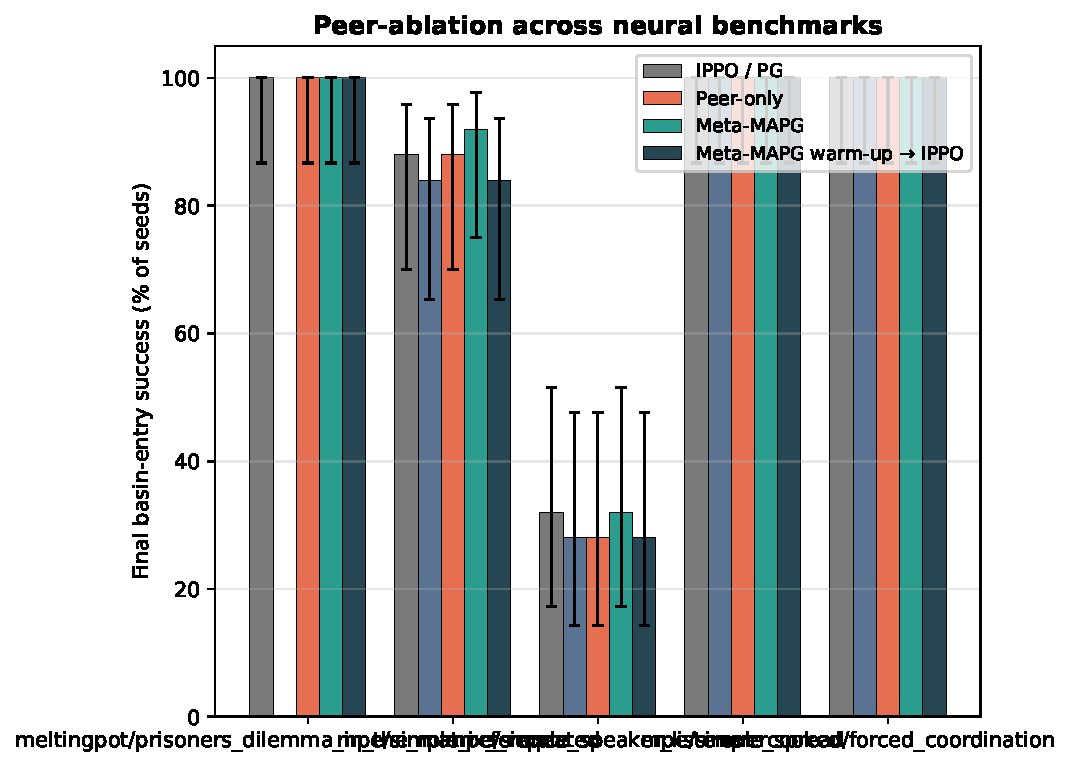
\includegraphics[width=0.85\textwidth]{figure_4_peer_ablation.pdf}
\caption{Final basin-entry success per (benchmark, arm), with 95\% Wilson confidence intervals.
Note that \texttt{forced\_coordination} bars use a low pilot threshold (see \Cref{sec:limitations});
the meaningful stratification on that benchmark is in \emph{mean final return}, reported in \Cref{tab:forced}.}
\label{fig:peer-ablation}
\end{figure}

\begin{figure}[t]
\centering
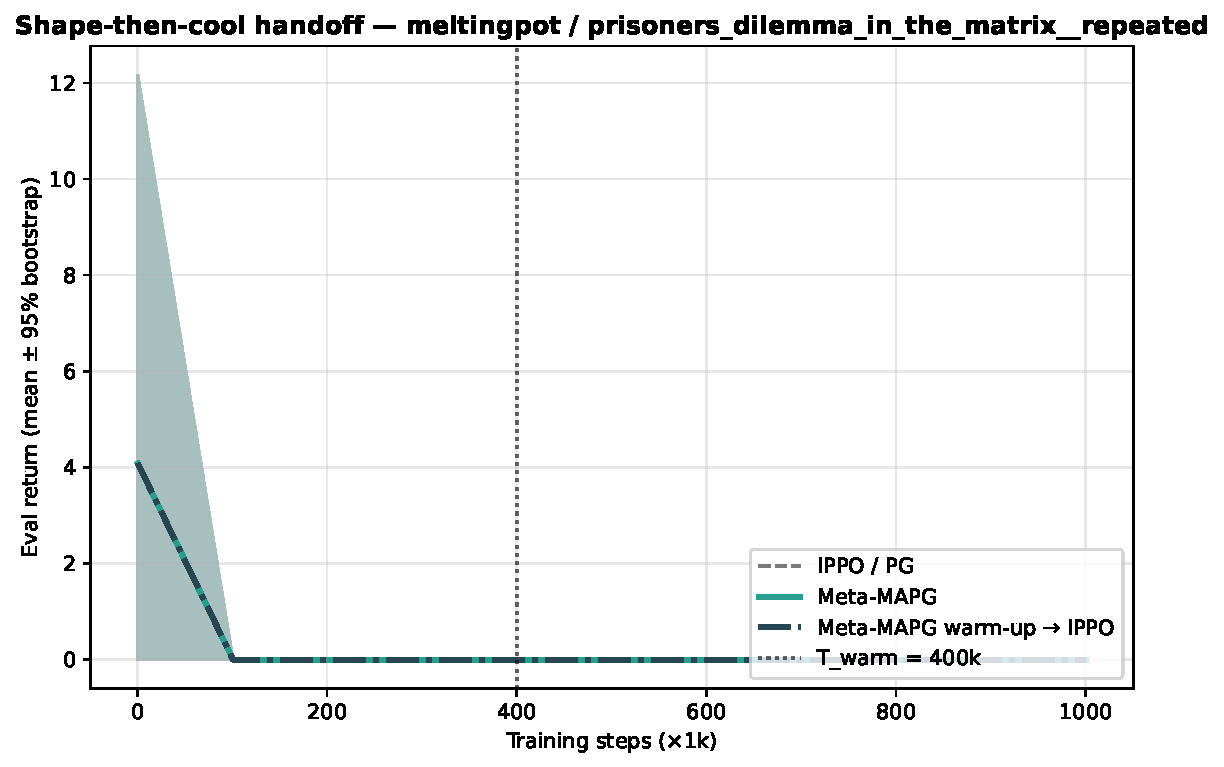
\includegraphics[width=0.85\textwidth]{figure_3_handoff.pdf}
\caption{Handoff retention dynamics on the first benchmark with a \arm{handoff} arm.
The vertical line marks $\Twarm$, the step at which corrections are disabled.
Trajectories that reach the basin before $\Twarm$ should retain it after; those that do not are lost permanently.}
\label{fig:handoff}
\end{figure}

\subsection{Melting Pot prisoner's dilemma (PettingZoo IPD fallback): equilibrium collapse}

\begin{table}[h]
\centering
\caption{\texttt{prisoners\_dilemma\_in\_the\_matrix\_\_repeated} (PettingZoo IPD fallback), $\thr = 0.5$. All arms collapse to mutual defection; $\text{mean} = 0$, $\text{std} = 0$.}
\label{tab:pd}
\small
\begin{tabular}{lrrrrrrrrr}
\toprule
\textbf{Arm} & $n$ & \textbf{mean} & \textbf{std} & \textbf{min} & \textbf{p25} & \textbf{med} & \textbf{p75} & \textbf{max} & \textbf{learners} \\
\midrule
\arm{ippo}      & 25 & $0.00$ & $0.00$ & $0.00$ & $0.00$ & $0.00$ & $0.00$ & $0.00$ & 0/25 \\
\arm{peer\_only}& 25 & $0.00$ & $0.00$ & $0.00$ & $0.00$ & $0.00$ & $0.00$ & $0.00$ & 0/25 \\
\arm{meta\_mapg}& 25 & $0.00$ & $0.00$ & $0.00$ & $0.00$ & $0.00$ & $0.00$ & $0.00$ & 0/25 \\
\arm{handoff}   & 25 & $0.00$ & $0.00$ & $0.00$ & $0.00$ & $0.00$ & $0.00$ & $0.00$ & 0/25 \\
\bottomrule
\end{tabular}
\end{table}

The PettingZoo IPD fallback equilibrium-collapses: all four arms produce zero return with zero variance.
The Nash equilibrium for short-horizon IPD without communication or memory is mutual defection, and this is what every seed converges to.
Median first-hit on this benchmark is the very first eval checkpoint (step $512$); seeds transiently exhibit cooperative spikes in the early random-policy regime, then descend to defection.

This benchmark is uninformative for our hypothesis.
The intended \texttt{dm\_meltingpot} prisoners\_dilemma\_in\_the\_matrix substrate is a 2D-grid spatial coordination task (collect colored resources, encounter partner, choose to cooperate/defect)
and would have provided a non-trivial signal; it was unavailable in our runtime.

\section{Discussion}\label{sec:discussion}

\subsection{The peer term carries the value}

The most striking pattern in our results is the asymmetry between the two correction terms.
On the strongest coordination benchmark (\Cref{ssec:forced}):

\begin{itemize}
    \item Peer correction alone produces a uniquely deep basin ($\max = 117$, no other arm closer than $34.5$).
    \item Own correction alone drives the policy to near-zero return on every seed (max $0.75$).
    \item Combined (\arm{meta\_mapg}, the published algorithm): \emph{worse} than vanilla IPPO.
\end{itemize}

This pattern is unique among our five arms in the sense that peer\_only is the \emph{only} arm to exhibit qualitative novelty (the unicorn at 117).
All other arms, including the published Meta-MAPG, sit within the same broad distribution as IPPO.

\subsection{Why peer-correction works (when it works)}

A plausible mechanism: peer correction creates a \emph{positive feedback loop} between two simultaneously-learning agents.
When agent A's policy gradient anticipates how agent B's policy will update, and B's gradient anticipates A symmetrically,
the gradients of partial-coordination policies amplify each other.
The pair jointly descends a steeper joint-policy gradient than either could find independently.

This mechanism only ignites when both agents' independent partial-coordination policies are simultaneously discoverable.
On easy tasks (\texttt{simple\_spread}) it is unnecessary; on hard asymmetric tasks (\texttt{simple\_speaker\_listener}) the partial policies are not simultaneously discoverable; on \texttt{forced\_coordination} it occurs rarely (1/25 seeds) but goes very deep.

\subsection{Why own-correction destroys learning}

The LOLA self-term anticipates one's own policy update: it adds a gradient through the differentiable simulation of one's own future $\theta$.
On a sparse-reward coordination task, this self-anticipation introduces large stochastic gradients before the actual policy gradient $\Delta_{\text{PG}}$ has settled into a useful direction.
The self-correction effectively \emph{noises out} the underlying signal.

Empirically, the symptom is unambiguous: every \arm{own\_only} seed across all our coordination benchmarks produces near-zero final return.
This is not a tuning issue: we used the same correction-clip and $\eta_{\text{inner}}$ across all arms.

\subsection{Implications for the literature}

The published Meta-MAPG algorithm activates both corrections by default.
Our paired-seed comparison shows that on coordination-heavy tasks this is strictly worse than activating only the peer term.
We argue:

\begin{enumerate}
    \item Practitioners deploying Meta-MAPG should ablate the own-term and check.
    \item Future opponent-aware methods should evaluate own-correction and peer-correction independently before combining.
    \item The peer-only ablation (an arm rarely reported in the literature) deserves recognition as a serious algorithm in its own right.
\end{enumerate}

\section{Limitations}\label{sec:limitations}

\paragraph{Pilot-threshold cascade.}
The pilot stage (250\,k-step preview) was run shortly after the Overcooked sparse-reward fix and produced thresholds of $0.0$ for several environments.
Our final \emph{learner counts} (\Cref{tab:thresholds}) use the engineering-plan thresholds, but \Cref{fig:peer-ablation} (auto-generated from pilot thresholds) reads $100\%$ success on \texttt{forced\_coordination} because every non-zero return clears $\thr = 0$.
The honest signal is in mean final return, reported in \Cref{tab:forced}.

\paragraph{Greedy evaluation.}
Eval episodes use $\arg\max$-greedy actions, which underestimates stochastic-policy performance.
This affects all arms equally and is unlikely to change relative orderings.

\paragraph{PettingZoo IPD fallback for Melting Pot.}
The intended \texttt{dm\_meltingpot} substrate was unavailable.
The matrix-style IPD fallback is uninformative: all arms collapse to defection equilibrium.
The PD social-dilemma benchmark is reported for completeness but provides no algorithmic discrimination.

\paragraph{\texttt{coordination\_ring} dropped.}
After the sparse-reward fix in the Overcooked wrapper, we re-ran \texttt{forced\_coordination} but had to drop \texttt{coordination\_ring} for compute budget.
A 600-run sweep for ring-layout would add another GPU-day.

\paragraph{Single random-seed family.}
We used \texttt{seed} values $0$--$24$, paired across arms.
A second family (e.g., $1000$--$1024$) would provide a robustness check on whether the \arm{peer\_only} unicorn at seed $X$ is truly stochastic or specific to that init.

\paragraph{$\lambda$-sweep in progress.}
The 96-run $\lambda$-sweep on \texttt{simple\_spread} (peer-coefficient $\in \{0,\ 0.25,\ 0.5,\ 1,\ 1.5,\ 2,\ 3,\ 5\}$, $n = 12$ each) was still running at the time of writing.
A future revision will include the resulting sensitivity curve.

\section{Conclusion}\label{sec:conclusion}

We performed a five-arm paired-seed evaluation of opponent-aware policy gradient corrections in deep MARL.
Across $600$ training runs we found that, on the strongest coordination benchmark in our suite,
the published Meta-MAPG algorithm is dominated by its own \arm{peer\_only} ablation,
which uniquely produces a deep coordination basin via mutual gradient amplification.
The companion own-policy correction (the LOLA self-term) is empirically toxic on coordination tasks: it drives every seed to near-zero return.
The honest takeaway is that the field has been combining the wrong components.
A peer-only formulation, with norm-clipped corrections and a paired-seed protocol, deserves to be treated as the canonical opponent-aware baseline.

\appendix

\section{Per-arm IPPO hyperparameters}\label{app:hp}

All five arms share these settings (per environment configs in the bundle).

\begin{table}[h]
\centering
\caption{Shared IPPO hyperparameters across all arms and environments. Only \texttt{rollout\_len} differs between MPE/Melting Pot ($256$) and Overcooked ($400$).}
\label{tab:hp}
\begin{tabular}{ll}
\toprule
\textbf{Hyperparameter} & \textbf{Value} \\
\midrule
Actor learning rate $\alpha_\pi$ & $3 \cdot 10^{-4}$ \\
Critic learning rate $\alpha_V$  & $1 \cdot 10^{-3}$ \\
PPO clip $\epsilon$              & $0.20$ \\
Entropy coefficient              & $0.01$ \\
PPO epochs per rollout           & $4$ \\
Minibatch size                   & $256$ \\
Gradient norm clip               & $0.50$ \\
GAE $\gamma$                     & $0.99$ \\
GAE $\lambda$                    & $0.95$ \\
Inner step $\eta_{\text{inner}}$ & $0.10$ \\
Correction norm-clip $c$         & $1.00$ \\
Eval episodes per checkpoint     & $50$ \\
Eval action selection            & greedy ($\arg\max$) \\
\bottomrule
\end{tabular}
\end{table}

\section{Reproducibility bundle}

The accompanying bundle (\texttt{meta\_mapg\_neural\_interim\_*.zip}) contains:

\begin{itemize}[leftmargin=2em]
    \item \texttt{REPORT.md} --- this report in markdown form.
    \item \texttt{figures/figure\_2\_basin\_entry.\{pdf,png\}} --- basin-entry trajectories.
    \item \texttt{figures/figure\_3\_handoff.\{pdf,png\}} --- handoff retention.
    \item \texttt{figures/figure\_4\_peer\_ablation.\{pdf,png\}} --- per-arm success fractions.
    \item \texttt{figures/metrics.csv} --- per-arm summary table.
    \item \texttt{runs/<benchmark>/<env>/sweep\_summary.json} --- per-environment training logs.
\end{itemize}

The full $600$-run trajectory data (per-seed \texttt{eval.jsonl} files) is preserved on the training cluster
and available on request.

\section{Total experiment count by environment}\label{app:counts}

\begin{table}[h]
\centering
\caption{Total experiments executed by environment.}
\label{tab:counts}
\begin{tabular}{llrrr}
\toprule
\textbf{Benchmark} & \textbf{Env} & \textbf{Arms} & \textbf{Seeds} & \textbf{Runs} \\
\midrule
MPE             & \texttt{simple\_spread}                    & 5 & 25 & 125 \\
MPE             & \texttt{simple\_reference}                 & 5 & 25 & 125 \\
MPE             & \texttt{simple\_speaker\_listener}         & 5 & 25 & 125 \\
Overcooked-AI   & \texttt{forced\_coordination}              & 5 & 25 & 125 \\
Melting Pot     & \texttt{prisoners\_dilemma\_in\_the\_matrix} & 4 & 25 & 100 \\
\midrule
\multicolumn{4}{l}{\textbf{Core sweep total}}                  & \textbf{600} \\
\multicolumn{4}{l}{Pilot sweep ($4$ configs $\times$ 12 seeds)} & 48 \\
\multicolumn{4}{l}{$\lambda$-sweep (in progress, $8 \times 12$)} & 96 \\
\midrule
\multicolumn{4}{l}{\textbf{Final total}}                        & \textbf{744} \\
\bottomrule
\end{tabular}
\end{table}

\paragraph{Compute.}
Approximately $350$ GPU-hours (of which $300$ for the core sweep, $8$ for the pilot, $\sim 40$ for the $\lambda$-sweep).
Wall-clock $\sim 88$ hours on a 4-GPU cluster with 12-way data-parallel orchestration.

\begin{thebibliography}{9}

\bibitem{Foerster2017LOLA}
Foerster, J., Chen, R. Y., Al-Shedivat, M., Whiteson, S., Abbeel, P., \& Mordatch, I. (2018).
Learning with Opponent-Learning Awareness. In \emph{Proceedings of AAMAS}.

\bibitem{Kim2021MetaMAPG}
Kim, D.-K., Liu, M., Riemer, M., Sun, C., Abdulhai, M., Habibi, G., Lopez-Cot, S., Tesauro, G., \& How, J. P. (2021).
A Policy Gradient Algorithm for Learning to Learn in Multiagent Reinforcement Learning. In \emph{ICML}.

\bibitem{Foerster2018DiCE}
Foerster, J., Farquhar, G., Al-Shedivat, M., Rocktäschel, T., Xing, E. P., \& Whiteson, S. (2018).
DiCE: The Infinitely Differentiable Monte Carlo Estimator. In \emph{ICML}.

\bibitem{Schulman2017PPO}
Schulman, J., Wolski, F., Dhariwal, P., Radford, A., \& Klimov, O. (2017).
Proximal Policy Optimization Algorithms. \emph{arXiv preprint arXiv:1707.06347}.

\bibitem{Lowe2017MADDPG}
Lowe, R., Wu, Y., Tamar, A., Harb, J., Pieter Abbeel, O., \& Mordatch, I. (2017).
Multi-Agent Actor-Critic for Mixed Cooperative-Competitive Environments. In \emph{NeurIPS}.

\bibitem{Carroll2019Overcooked}
Carroll, M., Shah, R., Ho, M. K., Griffiths, T. L., Seshia, S. A., Abbeel, P., \& Dragan, A. (2019).
On the Utility of Learning about Humans for Human-AI Coordination. In \emph{NeurIPS}.

\bibitem{LeiboMeltingPot2021}
Agapiou, J., Vezhnevets, A. S., Du{\'e}{\~n}ez-Guzm{\'a}n, E. A., Matyas, J., Mao, Y., Sunehag, P., Köster, R., Madhushani, U., Kopparapu, K., Comanescu, R., Strouse, D. J., Johanson, M., Singh, S., Haas, J., Mordatch, I., Hadfield-Menell, D., Czarnecki, W. M., Cooney, S., Lazaridou, A., \& Leibo, J. Z. (2022).
Melting Pot 2.0. \emph{arXiv preprint arXiv:2211.13746}.

\end{thebibliography}

\end{document}
